\chapter{Evaluation}
\label{cap:cap05}

In this chapter we evaluate our work in terms of the requisites presented on section \ref{sec:sec02}. The first section shows in numbers how many features are covered by the software switch. Subsequently, in the next section, we present the results of performance benchmarks tests. 


\subsection{Experimental Evaluation}
We propose two methods to evaluate our prototype: The first one focused in asses the functionality of the pipeline and controller, therefore, this evaluation will be present along BNG development with virtual interfaces, the second one is using our BNG software switch with MACSAD tool in a Linux server to run, compile and assess the performance in a real environment with 10G NIC. Details below:

\subsubsection{Functional Evaluation}
We assess the functionality of the control plane of the BNG software switch using a packet generator (Scapy) to generate and transmit packets through it and a network protocol analyzer (Wireshark) in a development environment to verify the sent and received packets along the virtual interfaces. The BNG functions to be evaluated are: 

\begin{itemize}
	\item Lookup tables
	\item L3 forwarding
	\item Mac learning
	\item Encap/Decap GRE header
	\item Network address translation
	\item Traffic manager 
	\item Controller functions like send entry tables
\end{itemize}

\subsubsection{Performance Evaluation}
\begin{itemize}
	\item It is important to judge the performance of  \acrshort{BNG} device, considering that we could have millions of packets trough it. 
	In order to validate the BNG software switch in a real network environment, we will compile on the Macsad tool in a commodity server, where the BNG software switch interfaces are connected to the Network Function Performance analyzer (NFPA \cite{nfpa}) node  via two 10G links to generates test traffic (See figure \ref{fig:bng_perf} ).
	
	
	\begin{figure}[ht]
		\centering
		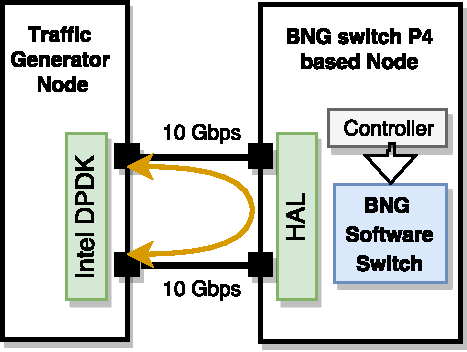
\includegraphics[width=0.35\linewidth] 
		{figures/bng_perf.pdf}
		\caption{BNG performance evaluation scenario.}
		\label{fig:bng_perf}
	\end{figure}
	
	This proof-of-concept implementation, will be run over Macsad server than will receive and forward the packets from Port 0 to Port 1, the NFPA node linked with MACSAD will send the packets and analyze the throughput in packets per second (pps) and bits per second (bps).\\
	
	For the BNG best-case test, the NFPA node will transmit packets with a fixed source and destination MAC addresses, and IP addresses, TCP port, and tunnel IP addresses, the configurations of the tables are presented,   in figure \ref{fig:bng_tables}
	For complex use case, the NFPA provides a wide selection of traffic traces with different packet headers and sizes,  for example with 1 to 1 million of packets with different flows and each one having different destination and source MAC addresses, different source and destination IP addresses, different TCP ports, different GRE IP addresses plus
	different source and destination port.
	
	\begin{figure}[ht]
		\centering
		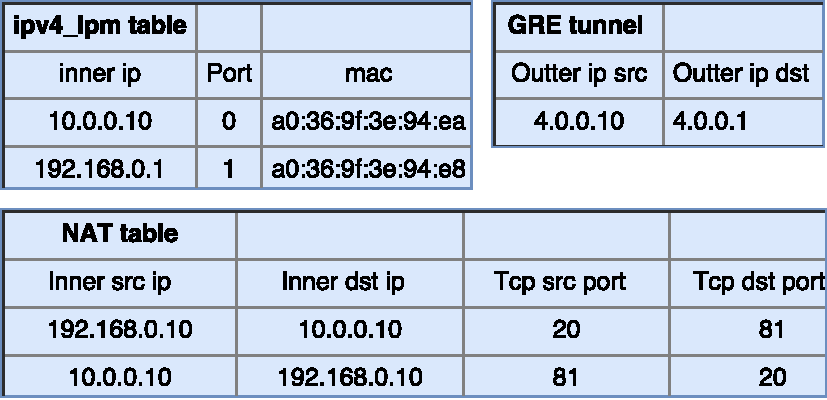
\includegraphics[width=0.6\linewidth] 
		{figures/bng_tables.pdf}
		\caption{Best-case Tables information.}
		\label{fig:bng_tables}
	\end{figure}
	
	
	
\end{itemize}



\section{Feature Completeness}
\label{sec:FeatureComplete}
Evaluating the proper operation of the BNG switch features is not a trivial task. For example, testing all flow match fields combinations would require creation of a large number of flows and packets, making manual tests very time consuming. For this reason, automatic test frameworks, discussed on section \ref{sec:testemulation}, are the best options to test the switch functionality in order to evaluate feature completeness.    

\section{Performance Benchmarks}

One of the software switch requirements listed on chapter \ref{cap:intro} is to reach a maximum throughput of at least 10Gb/s. For this reason we evaluated the switch performance in terms of network metrics. In this section we show how the switch performs for different packet sizes in comparison with different Pktio. Also, we investigated how performance is affected by the number of flows and by the number of tables traversed to match a packet.  

The machine configuration used to perform measurement tests are listed in the box below. 

\begin{framed}

\begin{itemize}
\item \textbf{Processor}:	8x Intel(R) Core(TM) i7-2670QM CPU @ 2.20GHz
\item \textbf{Memory}:	6003MB 
\item \textbf{Operating}: System	Ubuntu 16.04 LTS
\end{itemize}

\end{framed}

    \subsection{Maximum Throughput}
    \label{sec:MaxBand}
    This test evaluates the maximum forwarding rate the software switch can reach in comparison to other userspace implementations. 
    
    The setup for maximum throughput evaluation is the following:
    
    \begin{itemize}
    \item A running instance of the software switch with two virtual interfaces - Port 1 and Port 2 - attached. 
    \item One flow installed in the Flow Table to match a packet sent to Port 1 with destiny external network... The action is an output packet to Port 2. 
    \item A packet traffic generator. We used a NFPA tool  \cite{packeth}... .
    \item A script running in the Linux terminal checking the current packet rate on Port 2.   
    \end{itemize}
    
    The test starts by installing the flow in the switch Flow Table. Afterwards, we inject packets, using the traffic generator, directly into Port 1. The bandwidth results of Port 2, reported by the script, are used to calculate the maximum rate.  
    Two transmission measurements were made for 7 packet sizes: for packets of 64Kb, 128kb, 256kb, 512kb, 1024kb, 1280kb and bigger packets of 1500Kb. Figure \ref{graph:comparison} shows results for both experiments.

    
   Switch forwarding performance for small packets is evaluated in Kilo packets per second (Kpps). Figure \ref{graph:comparison64} shows that ofsoftswitch13 can handle xx.xx Kpps. This result is very 
   far from xxx and approximatelly 32\% more efficient than xxx. Bigger packets are measured in Megabits per second. Results presented in Figure \ref{graph:comparison1500} show that ... 
   
        
   
    
